\section{Insiemi}
\subsection{Simbologia}
Per indicare gli insiemi si utilizzano lettere maiuscole ($A, B, X, Y ...$). Per indicare gli elementi appartenenti ad un insieme si usano le lettere minuscole ($a, b, x, y ...$). Di seguito una lista di simboli necessari per lavorare con gli insiemi:

\begin{itemize}
    \item $\in$ \qquad Appartiene
    \item $\notin$ \qquad Non appartiene
    \item $\forall$ \qquad Per ogni
    \item $:$ \textit{or} $|$ \qquad Tale che
    \item $\exists$ \qquad Esiste (almeno)
    \item $\nexists$ \qquad Non esiste
    \item $\exists \oc$ \qquad Esiste ed è unico
    
    \item $\subseteq$ \qquad Inclusione insiemi
    \item $\subsetneqq$ \qquad Inclusione stretta (cioè $A \subseteq B$ e $A \neq B$)
    \item $\nsubseteq$ \qquad Non incluso
    
    \item $\bigcup$ \qquad Unione
    \item $\bigcap$ \qquad Intersezione
    \item $\emptyset$ \qquad Insieme vuoto
    \item $\setminus$ \qquad Meno tra insiemi
    \item $\mathbb{U}$ \qquad Insieme universale
    \item $\complement \left(A\right)$ \qquad Complementare di $A$ in $\mathbb{U}$, cioè tutti gli elementi di $\mathbb{U}$ che non sono in $A$ ($\complement \left(A\right) = \mathbb{U} \setminus A$).
    
    \item $\lor$ \qquad OR logico
    \item $\land$ \qquad AND logico
    \item $\implies$ \qquad Implica
    \item $\iff$ \qquad Coimplica, "se e solo se" 
\end{itemize}

\subsection{Preposizioni e utilizzo di simboli logici}
%VEDERE PREPOSIZIONI

Le \textbf{preposizioni} sono "frasi" che posso essere vere o false. Per legare due o più preposizioni si utilizzano i simboli logici $\land$ (and) e $\lor$ (or). %FARE MEGLIO

\begin{table}[H]
\centering
\begin{tabular}{|cc|c|c|c|}
\hline
p & q & \multicolumn{1}{l|}{p $\land$ q} & \multicolumn{1}{l|}{p $\lor$ q} & \multicolumn{1}{l|}{p $\implies$ q} \\ \hline
{\color[HTML]{000000} false} & {\color[HTML]{000000} false} & false & false & true \\
{\color[HTML]{000000} false} & {\color[HTML]{000000} true} & false & true & true \\
{\color[HTML]{000000} true} & {\color[HTML]{000000} false} & false & true & false \\
true & false & true & true & true \\ \hline
\end{tabular}

\caption{Tabella di verità per AND, OR e IMPLICAZIONE}
\end{table}

Nell'implicazione ($p \implies q$) $p$ è condizione sufficiente per $q$, mentre $q$ è condizione necessaria per $p$.

Se si vuole negare una preposizione si utilizza il simbolo di negazione ($^-$), quindi $p$ negato risulta $\overline{p}$. Di seguito alcune negazioni di simboli generali:
\begin{itemize}
    \item $\overline{\forall} = \exists$
    \item $\overline{\exists} = \forall$
\end{itemize}
Un esempio classico che si porta per comprendere la negazione: $p = $ \textit{lavoro tutti i giorni della settimana}, $\overline{p} =$ \textit{esiste almeno un giorno della settimana in cui non lavoro}.\\

È interessante notare che se si ha un'implicazione, si negano entrambe le preposizioni e si scambiano i termini il risultato rimane invariato.

\begin{table}[H]
\centering
\begin{tabular}{|cc|c|c|}
\hline
p & q & \multicolumn{1}{l|}{$p \implies q$} & \multicolumn{1}{l|}{$\overline{q} \implies \overline{p}$} \\ \hline
{\color[HTML]{000000} false} & {\color[HTML]{000000} false} & false & false \\
{\color[HTML]{000000} false} & {\color[HTML]{000000} true} & false & true \\
{\color[HTML]{000000} true} & {\color[HTML]{000000} false} & false & true \\
true & false & true & true \\ \hline
\end{tabular}
\caption{Implicazione con termini negati e invertiti}
\end{table}

Avendo la stessa tabella di verità $p \implies q = \overline{q} \implies \overline{p}$. Da qui nasce la \textbf{dimostrazione per negazione} (o contronominale). Esempio: se vogliamo dimostrare che se $n^2$ \textit{è pari} allora $n$ \textit{è pari}, ci basta dimostrare che se $n$ \textit{è dispari} allora $n^2$ \textit{è dispari} (Dimostrazione \ref{QuadratoDispari}). \label{dimostrazioneNegazione}

\subsection{Insiemi numerici noti}

\subsubsection{Naturali, interi e razionali}

Il primo insieme che si introduce è l'insieme dei \textbf{numeri naturali}, indicato con $\mathbb{N}$. Non definiremo formalmente l'insieme, ci basti sapere che comprende tutti i numeri interi positivi. È generalmente scritto nella forma:
\begin{center}
    $\mathbb{N} = \{0, 1, 2, 3, ...\}$
\end{center}
Gli elementi dell'insieme si indicano quindi tra parentesi graffe.\\

Il secondo insieme che va introdotto è quello dei \textbf{numeri interi}. Questo insieme comprende tutti i numeri che non hanno la virgola (per l'appunto interi) e si distingue da $\mathbb{N}$ in quanto ha al sui interno anche i numeri negativi. Il suo simbolo è $\mathbb{Z}$ e viene generalmente scritto come segue:
\begin{center}
    $\mathbb{Z} = \{..., -2, -1, 0, 1, 2, ...\}$
\end{center}

Non sempre però è comodo descrivere gli insiemi elencando il loro termini (in realtà non viene quasi mai fatto in quanto si creerebbero delle ambiguità). È necessario quindi utilizzare una notazione diversa per descrivere un insieme, ed è quello che si usa anche per introdurre $\mathbb{Q}$, l'insieme dei \textbf{numeri razionali}:
\begin{center}
    \begin{equation*}
        \mathbb{Q} = \left\{\,\dfrac{p}{q}\, \middle| \, p, q \in \mathbb{Z},\, q \neq 0 \right\}
    \end{equation*}
\end{center}
In questo caso l'insieme dei numeri razionali indica appunto l'insieme di tutte le frazioni (matematici rigorosi abbiate pietà della mia anima). E per esplicitarlo non cominciamo ad elencare tutte le frazioni, ma bensì utilizziamo una preposizione (?).\\ %DA CONTROLLARE

\subsubsection{Reali}
L'ultimo insieme che introduciamo è l'insieme dei \textbf{numeri reali}. Viene indicato con il simbolo $\mathbb{R}$ ed è l'insieme più importante di tutti i precedenti. Questo insieme viene introdotto perché all'insieme dei numeri razionali ($\mathbb{Q}$) mancano dei numeri.

Proviamo infatti a prendere una retta e a inserirci tutti i numeri che conosciamo per ora (cioè quelli contenuti in Q). Costruiamo ora un quadrato di lato 1, e proviamo a calcolare la lunghezza della sua diagonale con il teorema di Pitagora. Il numero che otterremo sarà $\sqrt{1^2+1^2} = \sqrt{2}$. Se proiettiamo questo numero sulla retta vediamo chiaramente che esiste un punto che corrisponde a $\sqrt{2}$.

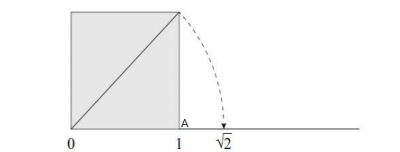
\includegraphics[]{img/sqrt2.png}

Questo punto è contenuto nell'insieme $\mathbb{Q}$? 

\pf{
    \textbf{Ipotesi}: $\sqrt{2} \in \mathbb{Q}$
    
    Se $\sqrt{2}$ è contenuta in $\mathbb{Q}$, questo significa che:
    
    \begin{equation*}
        \exists\, m, n, \in \mathbb{N} : \dfrac{m}{n} = \sqrt{2}
    \end{equation*}
    Cioè esistono due numeri appartenenti all'insieme dei numeri naturali tali che il loro rapporto è esattamente $\sqrt{2}$.
    
    Ovviamente essendo una frazione possiamo semplificare $m$ e $n$ fino ad eliminare tutti i loro fattori comuni, cioè fino a farli diventare \textbf{coprimi} o meglio $\mathrm{M.C.D}(m,n) = 1$.
    
    \begin{equation*}
        \dfrac{m}{n} = \sqrt{2} \implies \dfrac{m^2}{n^2} = \sqrt{2} \implies m^2 = 2n^2
    \end{equation*}
    Possiamo quindi dedurre che $m^2$ è pari, e quindi $m$ è pari (Dimostrazione \ref{QuadratoDispari}).
    Quindi $\exists\, k \in \mathbb{N} : m = 2k$.
    \begin{equation*}
        m^2 = 2n^2 \implies (2k)^2 = 2n^2 \implies 4k^2 = 2n^2 \implies 2k^2 = n^2
    \end{equation*}
    Quindi se $n^2$ è pari, anche $n$ è pari (Dimostrazione \ref{QuadratoDispari}).\\
    
    \textbf{Conclusione}: Abbiamo dimostrato che sia $m$ che $n$ sono pari, eppure per ipotesi $m$ e $n$ non hanno hanno fattori in comune. \textbf{CONTRADDIZIONE!}.\\
    
    \textbf{Tesi}: $\sqrt{2} \notin \mathbb{Q}$
    \hfill Q.e.d.
}

Come abbiamo dimostrato $\sqrt{2}$ non appartiene all'insieme dei numeri razionali. Inoltre si può dimostrare che $\forall\, n \in \mathbb{N} : n$ \textit{non è un quadrato perfetto} $\implies \sqrt{n} \notin \mathbb{Q}$. %Aggiungere anche la frazione che non è un quadrato perfetto?
Ne consegue che esistono infiniti punti sulla retta che non appartengono a $\mathbb{Q}$, e anzi è molto più probabile che facendo la radice di un numero si ottenga un numero che non è incluso in $\mathbb{Q}$ piuttosto che il contrario. Quindi se si vuole formalizzare una teoria dei limiti è necessario lavorare su un insieme non "bucato", cioè un insieme \textbf{continuo}.\\

La proprietà che infatti distingue e differenzia $\mathbb{R}$ da $\mathbb{Q}$ è proprio la continuità (non ci sono "buchi") e la completezza (tutti i punti sulla retta hanno associato un unico numero reale). Esiste infatti una \textbf{corrispondenza biunivoca} che associa tutti i punti della retta ai numeri reali.\footnote{Per approfondire il concetto di \textit{corrispondenza biunivoca} è necessario fare riferimento al capitolo legato alla funzioni.}
Per definire meglio la proprietà di completezza è necessario introdurre alcuni concetti:

\dfn{
    Dato $A \neq \emptyset$ e $A \subseteq R$
    \begin{enumerate}
        \item $M \in \mathbb{R}$ si dice \textbf{maggiorante} di $A$ se: $\forall\, a \in A : a \leq M$.
        \item $m \in \mathbb{R}$ si dice \textbf{minorante} di $A$ se: $\forall\, a \in A : m \leq a$.
        
        \item Se $A$ ammette un maggiorante è \textbf{superiormente limitato}.
        \item Se $A$ ammette un maggiorante è \textbf{inferiormente limitato}.
        \item Se $A$ ammettere un maggiorante e un minorante è \textbf{limitato}.
        
        \item $b \in A$ si dice \textbf{massimo} di $A$ se $\forall\, a \in A : a \leq b$.
        \item $c \in A$ si dice \textbf{minimo} di $A$ se $\forall\, a \in A : c \leq a$.
        
        \item Il più piccolo dei maggioranti si chiama \textbf{estremo superiore} di $A$. Si indicato con $\mathbf{sup}\,A$. Se il massimo esiste coincide con l'estremo superiore. Se l'insieme è superiormente illimitato si scrive $\mathbf{sup}\,A = +\infty$.
        \item Il più garnde dei minoranti si chiama \textbf{estremo inferiore} di $A$. Si indicato con $\mathbf{inf}\,A$. Se il minimo esiste coincide con l'estremo inferiore. Se l'insieme è inferiormente illimitato si scrive $\mathbf{inf}\,A = -\infty$.
        
        \item L'\textbf{insieme dei maggioranti} di $A$ si indica come $\mathrm{Mg}(A) = \{n \in \mathbb{R}\,|\, n$ è un maggiorante di $A\}$. Il minimo di questo insieme coincide con l'estremo superiore di $A$.
        \item L'\textbf{insieme dei minoranti} di $A$ si indica come $\mathrm{Mn}(A) = \{n \in \mathbb{R}\,|\, n$ è un minorante di $A\}$. Il massimo di questo insieme coincide con l'estremo inferiore di $A$.
    \end{enumerate}
}
La proprietà di \textbf{completezza} \label{completezzaR} di $\mathbb{R}$ è quindi formalizzata nella seguente forma:
\imp{\begin{center}
    Dato un insieme limitato, esiste sempre un estremo inferiore e un estremo superiore.
\end{center}}

Per esempio, dato l'insieme $A = \{q \in \mathbb{Q}\,|\,q^2 < 2\}$ non è possibile trovare un estremo superiore e un estremo inferiore in quanto l'intervallo (sezione \ref{intervalli}) dell'insieme sarebbe $]-\sqrt{2}, \sqrt{2}[$ e, come dimostrato precedentemente, $\sqrt{2} \notin \mathbb{Q}$. Se invece si considera l'insieme $B = \{q \in \mathbb{R}\,|\,q^2 < 2\}$, è facile notare che $\mathrm{sup}\,A = \sqrt{2}$ e che $\mathrm{inf}\, A = -\sqrt{2}$.

\subsection{Intervalli} \label{intervalli}
Per indicare gli intervalli generalmente si utilizza una notazione con le parentesi. Viene utilizzata la parentesi quadra ($[$ e $]$) per indicare rispettivamente se un estremo dell'intervallo è compreso o no. In particolare se l'apertura della parentesi è rivolta verso il numero, allora tale numero è compreso. Di seguito degli esempi per chiarire. Gli intervalli sono comunque un insieme di punti e quindi questo si può tradurre:
\begin{itemize}
    \item $[a, b] = \left\{ x \in \mathbb{R}\, \middle|\, a \leq x 	\leq b\right\}$
    \item $]a, b] = \left\{ x \in \mathbb{R}\, \middle|\, a < x \leq b\right\}$
    \item $[a, b[ = \left\{ x \in \mathbb{R}\, \middle|\, a \leq x < b\right\}$
    \item $]a, b[ = \left\{ x \in \mathbb{R}\, \middle|\, a < x < b\right\}$
    
    \item $]-\infty, a] = \left\{ x \in \mathbb{R}\, \middle|\, a \leq x \right\}$
    \item $[b, +\infty[ = \left\{ x \in \mathbb{R}\, \middle|\, x \geq b \right\}$
    \item $]-\infty, +\infty[ = \mathbb{R}$
\end{itemize}
Con infinito si utilizza sempre la parentesi di esclusione. In alcuni libri viene utilizzata però la parentesi tonda: al posto di $[a,+\infty[$ viene scritto $[a. +\infty)$.

\subsection{Prodotto cartesiano}
\dfn{
    Dati due insiemi $A$ e $B$, il \textbf{prodotto cartesiano tra $A$ e $B$} si definisce come:
    \begin{equation*}
        A\times B = \{(a, b)\,|\,a \in A \land b \in B\}
    \end{equation*}
}

È quindi l'insieme di coppie ordinate ($(1, 0) \neq (0, 1)$). Attenzione che non vale la proprietà commutativa: $A\times B \neq B\times A$. Un prodotto cartesiano con lo stesso insieme si può abbreviare come $A^2 = A\times A$.\\ 

$\mathbb{R}$ = Retta. $\mathbb{R}^2$ = Piano cartesiano. $\mathbb{R}^3$ = Sistema di coordinate a tre dimensioni. %FARE GRAFICO

\subsection{Cardinalità}
La cardinalità per essere introdotta ha bisogno di alcune nozioni riguardo le funzioni. È consigliato quindi andare a vedere la sezione \ref{funzioni} e poi tornare qui.\\

\dfn{
    Dati due insiemi $A$ e $B$, se esiste una funzione biunivoca $f: A \to B$ si dice che \textbf{$A$ e $B$ sono equipotenti}.
}

\dfn{
    Due insiemi hanno la stessa cardinalità se sono equipotenti. Per indicare la cardinalità dell'insieme $A$ si scrive:
    \begin{equation*}
        |A|
    \end{equation*}
}

La cardinalità, in parole povere, è un modo per "misurare" e classificare gli insiemi in base a quanti elementi contengono. Se infatti abbiamo tre insiemi \textit{finiti} $A=\{1, 3, 5\}$, $B=\{2, 4, 6\}$ e $C=\{1, 2\}$ possiamo dire che A e C NON hanno la stessa cardinalità ($|A|=3 \neq |C| = 2$), mentre A e B hanno la stessa cardinalità ($|A| = |B| = 3$). Quindi la cardinalità riguardo insiemi \textit{finiti} si limita a misurare gli elementi che contengono gli insiemi stessi, mentre la cardinalità con insiemi \textit{infiniti} ci permette di capire quali insiemi contengono più elementi di altri (nonostante siano infiniti).\\

\subsubsection{Cardinalità del numerabile}

La cardinalità infinita \textit{più piccola} è la \textbf{cardinalità del numerabile}, cioè la stessa cardinalità dell'insieme dei numeri naturali ($|\mathbb{N}| = numerabile$).

Ora prendiamo in considerazione il secondo insieme che abbiamo introdotto subito dopo $\mathbb{N}$, cioè $\mathbb{Z}.$ L'intuito ci dice che la cardinalità dell'insieme dei numeri interi dovrebbe essere doppia rispetto a quella dei naturali, in quanto ci sono esattamente il doppio dei numeri (cioè anche i negativi oltre ai positivi). Proviamo però a definire una funzione $f: \mathbb{N} \to \mathbb{Z}$ tale che:

\begin{equation*}
    f(n) =
    \begin{cases}
    n/2 \qquad \quad \;\;\; \text{se $n$ è pari}\\
    -\dfrac{n+1}{2} \qquad \text{se $n$ è dispari}
    \end{cases}
\end{equation*}

I valori della funzione risultano quindi:
\begin{align*}
    f(0) = 0 \qquad \qquad f(1) = -1\\
    f(2) = 1 \qquad \qquad f(3) = -2\\
    f(4) = 2 \qquad \qquad f(5) = -3\\
    \vdots \qquad \qquad \qquad \qquad \vdots \qquad
\end{align*}

È facile notare che $f$ è biunivoca e, conseguentemente alle definizioni appena date, possiamo affermare che $\mathbb{Z}$ ha cardinalità del numerabile:
\begin{equation*}
    |\mathbb{Z}| = |\mathbb{N}|
\end{equation*}

Prendiamo ora in analisi l'insieme dei numeri razionali, ovvero $\mathbb{Q}$. Elenchiamo tutte le frazioni (e di conseguenza tutti i sui elementi) nel seguente ordine:

\begin{figure}[H]
\centering
\begin{tikzpicture}
% the matrix entries
\matrix (mat) [table]
{
0 & 1 & 2 & 3 & 4 & 5 & 6 & \dots \\
-0 & -1 & -2 & -3 & -4 & -5 & -6 & \dots \\
$ +\frac{0}{2}$ & $ +\frac{1}{2}$ & $ +\frac{2}{2}$ & $ +\frac{3}{2}$ & $ +\frac{4}{2}$ & $ +\frac{5}{2}$ & $ +\frac{6}{2}$ & \dots \\
$ -\frac{0}{2}$ & $ -\frac{1}{2}$ & $ -\frac{2}{2}$ & $ -\frac{3}{2}$ & $ -\frac{4}{2}$ & $ -\frac{5}{2}$ & $ -\frac{6}{2}$ & \dots \\
$ +\frac{0}{3}$ & $ +\frac{1}{3}$ & $ +\frac{2}{3}$ & $ +\frac{3}{3}$ & $ +\frac{4}{3}$ & $ +\frac{5}{3}$ & $ +\frac{6}{3}$ & \dots \\
$ -\frac{0}{3}$ & $ -\frac{1}{3}$ & $ -\frac{2}{3}$ & $ -\frac{3}{3}$ & $ -\frac{4}{3}$ & $ -\frac{5}{3}$ & $ -\frac{6}{3}$ & \dots \\
\vdots &\vdots &\vdots &\vdots &\vdots &\vdots &\vdots &\\
};
% the matrix rules

% the arrows
\begin{scope}[shorten >=7pt,shorten <= 7pt]
\draw[->]  (mat-1-1.center) -- (mat-1-2.center);
\draw[->]  (mat-1-2.center) -- (mat-2-1.center);
\draw[->]  (mat-2-1.center) -- (mat-2-2.center);
\draw[->]  (mat-2-2.center) -- (mat-1-3.center);
\draw[->]  (mat-1-3.center) -- (mat-1-4.center);
\draw[->]  (mat-1-4.center) -- (mat-2-3.center);
\draw[->]  (mat-2-3.center) -- (mat-3-2.center);
\draw[->]  (mat-3-2.center) -- (mat-3-1.center);
\draw[->]  (mat-3-1.center) -- (mat-4-1.center);
\draw[->]  (mat-4-1.center) -- (mat-4-2.center);
\draw[->]  (mat-4-2.center) -- (mat-3-3.center);
\draw[->]  (mat-3-3.center) -- (mat-2-4.center);
\draw[->]  (mat-2-4.center) -- (mat-1-5.center);
\draw[->]  (mat-1-5.center) -- (mat-1-6.center);
\draw[->]  (mat-1-6.center) -- (mat-2-5.center);
\draw[->]  (mat-2-5.center) -- (mat-3-4.center);
\draw[->]  (mat-3-4.center) -- (mat-4-3.center);
\draw[->]  (mat-4-3.center) -- (mat-5-2.center);
\draw[->]  (mat-5-2.center) -- (mat-5-1.center);
\draw[->]  (mat-5-1.center) -- (mat-6-1.center);
\draw[->]  (mat-6-1.center) -- (mat-6-2.center);
\draw[->]  (mat-6-2.center) -- (mat-5-3.center);
\draw[->]  (mat-5-3.center) -- (mat-4-4.center);
\draw[->]  (mat-4-4.center) -- (mat-3-5.center);
\draw[->]  (mat-3-5.center) -- (mat-2-6.center);
\draw[->]  (mat-2-6.center) -- (mat-1-7.center);
\end{scope}
\end{tikzpicture}

\caption{Tabella numeri razionali}
\label{TabellaNumeriRazionali}
\end{figure}

Non dimostreremo rigorosamente la cosa, però è facile notare che si può costruire una funzione biunivoca da $\mathbb{N}$ a $\mathbb{Q}$ che segua esattamente l'ordine delle frecce nella figura \ref{TabellaNumeriRazionali}. Di conseguenza anche l'insieme dei numeri razionali ha \textbf{cardinalità del numerabile}:
\imp{
\begin{equation*}
    |\mathbb{N}| = |\mathbb{Z}| = |\mathbb{Q}|
\end{equation*}
}

\subsubsection{Cardinalità del continuo} %DA FORMULARE MEGLIO
Concludiamo con l'analisi dei numeri reali, ovvero l'insieme $\mathbb{R}$. Se volessimo dimostrare che $|\mathbb{R}|$ non è numerabile, ci basterebbe dimostrare che un suo sottoinsieme non è numerabile. Proviamo quindi a dimostrare che l'intervallo $[0, 1[$ non è numerabile, cioè ha cardinalità maggiore dell'insieme dei numeri naturali ($\mathbb{N}$). Prendiamo tutti i numeri contenuti nell'intervallo $[0,1[$ e cominciamo ad elencarli senza un ordine preciso:
\begin{align*}
    0.1298417824611040752 \dots\\
    0.3793921999397529387 \dots\\
    0.2384798342293874812 \dots\\
    0.0073820271308387362 \dots\\
    0.4579468274062944976 \dots\\
    0.7432686162126636901 \dots\\
    \vdots \qquad \qquad \qquad
\end{align*}
Immaginiamo una funzione $f: \mathbb{N} \to [0,1[$ che associ ad ogni numero elencato un numero naturale. Ora indichiamo con $b_{ij}$ la cifra $j$ (partendo dai decimali) del numero $i$ e creiamo un nuovo numero $r$ secondo la regola:
\begin{equation*}
    r_{jj} = 
    \begin{cases}
    5 \qquad \mathrm{se}\;\,b_{jj} \neq 5\\
    6 \qquad \mathrm{se}\;\,b_{jj} = 5\\
    \end{cases}
\end{equation*}
È facile notare che $r$ è un numero diverso per almeno una cifra da tutti quelli elencati in precedenza. Ne consegue che non c'è nessun numero in $\mathbb{N}$ associato ad $r$, quindi $|\mathbb{R}|$ \textbf{non è numerabile}, infatti:
\imp{\begin{center}
    $\mathbb{R}$ ha \textbf{cardinalità del continuo}.
\end{center}}